\documentclass{article}
\usepackage{amsmath}
\usepackage{amssymb}
\usepackage{graphicx}
\usepackage{hyperref}
\usepackage[version=4]{mhchem}

\title{Problem 3}
\date{}

\begin{document}
\maketitle

\section*{Problem}
As shown in the figure, \(\triangle A B C\) is a right triangle with \(\angle C=90^{\circ} . A C\) is the diameter of circle \(O\). Circle \(O\) meets the hypotenuse \(A B\) at \(D\). Draw the tangent through \(D\) to the circle to meet the leg \(B C\) at \(E\). Prove: \(B E=E C\).\\
\centering
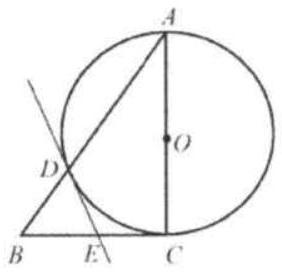
\includegraphics[width=\textwidth]{images/problem_image_1.jpg}

\section*{Solution}
Connect CD.


Since \(A C\) is the diameter, \(\angle A D C=90^{\circ}\).\\
Let \(\angle A=\alpha, \angle A C D=\beta\).\\
Then \(\angle E D C=\angle E C D=\angle A=\alpha\) (they all face the same \(\operatorname{arc} D C\) ).\\
Since \(\angle A C B=90^{\circ}, \angle B=\beta\).\\
Since \(\angle B D C=90^{\circ}, \angle B D E=\beta\).\\
Note that both \(E C\) and \(E D\) are tangent to the circle \(O, E D\)\\
\centering
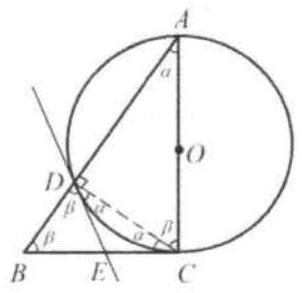
\includegraphics[width=\textwidth]{images/reasoning_image_1.jpg}\\
\(=E C\).\\
Thus \(D E=B E=E C\).

\end{document}
